
\chapter{Introduction and Objectives}

\label{Intro} 

%%% Introduction and Objectives: This chapter should set the scene for the reader. It must outline the background to the problem, give your reasons for the choice of project, and identify the project’s beneficiaries. Your objectives need to be precisely stated, together with the tests that will show, at the end of the project, that they have been met (or not been met). You need also to outline your methods in broad terms, along with y work plan with sufficient detail to show how you planned to meet the objectives. Outline any major changes of goals or methods that happened during the project. Finally, outline the structure of the report, showing how it fits together.

%-----------------------------------
%	BACKGROUND
%-----------------------------------

\section{Background}

% Chammas - 503 words, 7 references
% references
% 1. Self driving robot with Mainframe processor
% 2. European investment, Dickmans
% 3. Carnegie Melon
% 4. Darpa
% 5. Dave
% 6. NVIDIA

% Paragraph 1
% The goal of self driving cars...
% Self-driving cars are a difficult problem to solve...

% Paragraph 2
% With advances in deep learning, training algorithms and computational power...
%% Research question
%% Given the above, how reliable are self-driving cars relying on end-to-end ConvNets in the rain?
%% This project builds on something or other, uses natural and synthetic datasets

% What motivates the study of autonomous vehicles
The development of self-driving cars, a particular case of autonomous vehicle (AV), is motivated by a number of goals, of a practical, safety, public interest and economic nature.
%% Practical goal
 From a practical perspective, the goal is "to transport people from one place to another without any help from a driver" (\cite{s20092544}).
 %% Public health perspective
 From a public health perspective, to
transform the current approach
to automotive safety from reducing injuries after collisions to
 complete collision prevention (\cite{Fleetwood_2017}).
%% Business models
From a public interest and economic perspective, AV fleets allow for new shared autonomous mobility business models 
(\cite{riggs2019business})
though shared autonomous electric vehicle (SAEVs) fleets (\cite{loeb2019fleet}). Shared Autonomous Vehicles (SAVs) have gained significant public interest as a possible less expensive, safer and more efficient version of today’s transportation networking companies (TNCs) and taxis.

%% Perceived superiority of AV systems
This perceived superiority to human drivers is attributed to high-performance computing that allows AVs to process, learn from and adjust their guidance systems according
to changes in external conditions at much faster rates than the typical human driver  (\cite{west2016moving}).
%and it
%is supplemented with vehicle-to-vehicle (V2 V) and vehicle-to-infrastructure (V2I) %communication, allowing AVs to learn from other vehicles (\cite{west2016moving}).

% moved to reflections
%% Ethical issues - maybe leave to discussion and further work
%This also raises issues related to safety, liability, privacy, cybersecurity, and industry %risks \cite{Taeihagh_2018}
% TODO - how fast does the human eye process an image? How fast does a modern onboard AV system process and image

%% Sensor fusion approach
The self-driving system for AVs can be distinguished by two approaches: the multi-sensor pipeline approach (\cite{Grigorescu_2020}, \cite{Yurtsever_2020}) relying on data from radar, sonar, lidar and images,
%% End to end approach
and the end to end approach (\cite{bojarski2016end}), relying on images alone. 

Although CNNs have been successfully used to solve problems applied to Computer Vision, the robustness of such architectures has been increasingly scrutinised. \cite{Su_2019} proposed an algorithm where a deep neural network, when presented with a images (in this case images from the \cite{CIFAR_10} dataset) modified with a single pixel change, is capable of "fooling the network, such that an incorrect label is predicted with a high confidence value.  


%% In the context of overfitting:
\cite{zhang2017understanding} debated the need to rethink generalization, by demonstrating how traditional benchmarking approaches fail to explain why large neural networks generalize well in practice. By randomizing target labels, the experiments show that state-of-the-art convolutional neural networks for image classification trained with SGD (stochastic gradient descent) are large enough to fit a random labelling of the training data. This is achieved with a simple two-layer neural network, which presents a "perfect finite sample expressivity" as soon as the number of parameters exceeds the number of data points as usually is the case in practice with CNNs.  
This poses a challenge for self-driving cars, specially if relying only on images. Since testing real life scenarios is not practical in this study, two options are examined: using public self-driving datasets containing images labelled with steering angles, and using game engines (\cite{cowan2014survey}), which are capable of generating labeled datasets and realistic environments where the autonomous vehicle may be tested.
The research question is \textit{do images containing rain-like patterns affect self-driving CNNs trained to output steering predictions}? 

%-----------------------------------
%	AIMS AND OBJECTIVES
%-----------------------------------
\section{Aims and Objectives}

% Chammas - 165 words, no references

The main aim of this project is to to answer the research question, by evaluating how reliable are self driving cars using end to end convolutional neural network architectures to predict steering given images with rain-like noisy patters. The significance of this type of network is it relies only on raw pixel values, and no additional sensor inputs. 
To reach this aim, the project objectives are:
\begin{itemize}
    \item[--] Determine a game engine capable of supporting the experiments 
    \item[--] Select and create appropriate datasets 
    \item[--] Determine software packages able to augment and add rain-like patterns to digital images
    \item[--] Train self-driving end to end CNN models    
    \item[--] Establish a workflow to modify images to be presented to the network during the running (driving) phase
    \item[--] Determine a metric for evaluating how well a self-driving CNN is performing with respect to a steering ground truth    
\end{itemize}

%-----------------------------------
%	BENEFICIARIES
%-----------------------------------
\subsection{Beneficiaries}

% Chammas - 79 words, no references

Autonomous vehicles and robotics increasingly rely on computer vision and in some cases convolutional neural networks. The issue of reliability in computer vision based systems when faced with noisy data, in the case of this study, images containing rain, is one that affects any CNN based system, not only autonomous vehicles, hence, any findings in this work could be beneficial to help, practitioners inform design decisions, and industry approval bodies surveying benchmarking methodologies. The project, once reaching the aims, provides an open framework which may benefit any further research.

%-----------------------------------
%	Introduction to Methods and Work Plan
%-----------------------------------

\section{Introduction to Methods and Work Plan}

% Chammas - 130 words, no references

The work plan is to survey the literature for current trends in AV CNNs. Followed by researching required tools and datasets to create a development environment for training and testing. Then existing CNN self-driving models will be replicated and modified. Once results are produced a performance metric will assess individual models producing the metrics required to complete the report. 
The methods include the use of game engines to generate data and eare required are a game engine able to simulate select datasets and tools: a game engine and data augmentation library. then develop self-driving CNN models, then  determine model evaluation with a selected metric. And evaluate models quantitavely with the selected metric, and also qualitatively when using the game engine, by observing the self-driving vehicle around a simulated track and noting any oversterring and crashes.



%%%%%%%%%%%%%%%%%%%%%%%%%%%%%%%%%%%%%%
%	Changes in Methods and Work Plan
%%%%%%%%%%%%%%%%%%%%%%%%%%%%%%%%%%%%%%

\subsection{Changes in Methods and Work Plan}

% Chammas - 104 words, 1 reference, one image with revised work plan

% TODO There might not be enough time to get all proposed models working, so this section will be completed in the final week or two.
 
% Dec 7 we were still creating models 
% $ git show df953d2
%commit df953d22e72452116fd9416e8d283498c23f6c4f
%Author: Daniel Sikar <dsikar@gmail.com>
%Date:   Mon Dec 7 19:30:26 2020 +0000
%    Restored last 10 unit layer in nvidia2

% Dec 6 still augmenting data
% $ ls -lt Augmentation.py 
% -rw-rw-r-- 1 simbox simbox 6102 Dec  6 20:34 Augmentation.py

% Date on output folders for synthetic data show July and November

The original work breakdown structure described in appendix \ref{app:rpmi} was revised as shown in Figure \ref{fig:Revised-work-breakdown-structure}. 

\begin{figure}[ht]
 \centering 
 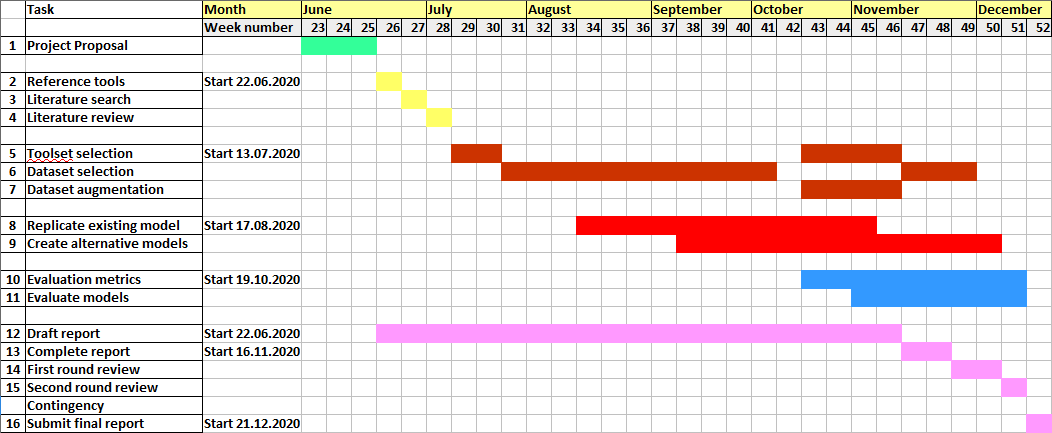
\includegraphics[width=\textwidth]{Figures/Revised-work-breakdown-structure.png}
 \caption{Retrospectively revised project work plan.}
 \label{fig:Revised-work-breakdown-structure} 
\end{figure}

%-----------------------------------
%	Structure of the report
%-----------------------------------

\section{Structure of the Report}

% Chammas - 324 words, no references
The remaining report is structured as follows:
\begin{itemize}
    \item[--] Chapter 2 provides the critical context, project motivation, methods used, literature survey and analysis. It outlines the current state of research with autonomous vehicles deep neural networks, including ConvNets.
    \item[--] Chapter 3 contextualises the broader context of self-driving cars and the technologies pushing research further
    \item[--] Chapter 4 describes results of training networks, together with metrics and video links showing the simulated car models self-driving
    \item[--] Chapter 5 contains a discussion on what objectives were met, then it assess how the results could be employed in other cases related to AVs and to computer vision and robotics in genral.
    \item[--] Chapter 6 evaluates and reflects on the project, limitations, contributions and ares for further work.
    \item[--] Appendix A contains the RPMI project proposal
    \item[--] Appendix B details methods used 
    \item[--] Appendix C contains network architectures used
    \item[--] Appendix D presents tables containing \textit{deliverables} first put forward to project supervisor
    \item[--] Appendix E contains training logs and notes on gathering results
    \item[--] Appendix F contains a list of outputs generated by this project
    \item[--] Appendix G contains listings for original and modified (with attribution) codes used in this project
    \item[--] This document in pdf format and a readme.txt file are submitted in the project submission area. readme.txt file lists SharePoint links for trained models, dataset, source code for training, testing, driving simulator and source code audit files.
\end{itemize}
